\documentclass[12pt,letterpaper,answers]{exam}
%\usepackage{color}
\usepackage[usenames,dvipsnames,svgnames,table]{xcolor}
\usepackage[margin=0.9in]{geometry}
\renewcommand{\familydefault}{\sfdefault}
\usepackage{multicol}
\pagestyle{head}
\definecolor{c02}{HTML}{FFBBBB}
\definecolor{c03}{HTML}{FFDDDD}
\header{AM 108 Problem Set 07}{}{{\colorbox{c02}{\makebox[3.0cm][l]{Due Fri Mar 24}}}\\ at noon p.\thepage}
\runningheadrule
\headrule
\usepackage{diagbox}
\usepackage{graphicx} % more modern
%\usepackage{subfigure} 
\usepackage{amsmath} 
\usepackage{amssymb} 
%\usepackage{gensymb} 
%\usepackage{natbib}
\usepackage{hyperref}
%\usepackage{enumitem}
%\setlength{\parindent}{0pt}
%\usepackage{setspace}
%\pagestyle{empty}  
%\newcommand{\Sc}[0]{
%{\color{BlueViolet}\S}
%}
\usepackage{tcolorbox}
\usepackage[framed,numbered,autolinebreaks,useliterate]{mcode}

% \renewcommand{\labelenumii}{\theenumii}
% \renewcommand{\theenumii}{\theenumi-\arabic{enumii}.}

\newif\ifprintselans
\printselanstrue
%\printselansfalse
\newenvironment{selans}
{\ifprintselans
   \printanswers
   \renewcommand{\solutiontitle}{\noindent\textbf{Answer:}\par\noindent}
 \fi
}
{}

\newif\ifprintselsol
%\printselsoltrue
\printselsolfalse
\newenvironment{selsol}
{\ifprintselsol
   \printanswers
   \renewcommand{\solutiontitle}{\noindent\textbf{Solution:}\par\noindent}
 \fi
}
{}


\begin{document}
 \pdfpageheight 11in 
  \pdfpagewidth 8.5in

\noindent\textbf{Problem Set Instructions:}  
\begin{itemize}
\itemsep0pt
\item In your first attempt of the problem set problems, you are encouraged to treat the problem set as an open-notes quiz.  Work on it without consulting classmates, Ed, course staff, other people, other internet resources, or any solutions or answers.  Work on each problem, completing as much as you are able to, and making a note in your work whenever you become stuck or confused.
\item After your initial individual attempt, collaboration is encouraged (see guidelines below) as you continue to work on the problems.  You'll submit a pdf of this work as part of your problem set submission on Gradescope (and will also submit it on Canvas).
\item Submit the pdf of your problem set work with the problems written up in order (computational work should be included: it can be at the end of the pdf) on Canvas and access the solutions.
\item Complete the reflection questions below, and submit that reflection work, along with your problem set pdf, on Gradescope.
\end{itemize}
  
\noindent\textbf{Submission Instructions:}  
\begin{itemize}
\item Following the instructions above, upload a pdf of your work to Canvas.  Upload your reflection answers and the pdf to Gradescope.
\item If you would like to use mathematical software other than Mathematica, that's fine. 
\end{itemize}

\noindent\textbf{Late Work Policy:}
\begin{itemize}
\itemsep0pt
\item Problem sets are accepted up to eight hours late with no penalty (8pm Friday). 
\item Three 36 hour late days are available to every student (three extensions to 8pm on Saturday).  These late days are expected to be used for unexpected illness or other conflicts.
\item Additional late days are not typically 
available.
\item Problem sets are not accepted beyond the late deadline.
\end{itemize}

\noindent\textbf{Collaborating on Problem Sets:}  

\noindent Collaborating with classmates in planning and designing solutions to homework problems is encouraged.  Collaboration, cooperation, and consultation can all be productive.  Work with others to: 
\begin{multicols}{2}
\begin{itemize}
\itemsep-0.2em
    \item discuss the problem
    \item brainstorm
    \item walk through possible strategies
    \item outline solution methods
\end{itemize}   
\end{multicols}

\noindent For homework, you may consult or use:
\begin{multicols}{2}
\begin{itemize}
\itemsep-0.2em
    \item Course text (including answers in back)
    \item Your notes (taken during class)
    \item Class notes of other students
    \item Course handouts
    \item Canvas posts/Ed posts
    \item Computational tools such as Python, Mathematica, or Desmos
    \item Calculators
    \item Other books
    \item the Internet
\end{itemize}
\end{multicols}

\noindent You may:
\begin{itemize}
    \item Look at communal work while writing up your own solution
\end{itemize}

\noindent You may \textbf{not}:
\begin{itemize}
\itemsep-0.2em
    \item Look at the individual work of others while writing up your own solutions
    \item Post about problems online
\end{itemize}


\noindent Do \textbf{not} consult the following resources until after you think you have solved a problem, have fully written up your answer, and have submitted a pdf of your work to Canvas.
%\begin{multicols}{2}
\begin{itemize}
\itemsep-0.2em
    \item The text solution manual
    \item The posted solutions
    \item Other solutions (from previous years, from sites like Chegg or Math Stackexchange, etc)
\end{itemize}
%\end{multicols}


%\eject


% \begin{enumerate}
% \item Reflection questions

\section*{Reflection questions}
Submit these on Gradescope.
\begin{enumerate}
\item \begin{enumerate}
    \itemsep0pt
    \item When you worked on the problems individually, how did each problem go?
    \item Where did you get stuck or confused?  For any subpart where you were stuck or confused be specific.  \emph{For example 'I tried to use the hint for 3b, but I couldn't find a way to relate $r$ and $x$'.}
    \item What additional progress were you able to make when you consulted other people or additional resources?
    \item For each part of each problem, how did your work compare with the posted solution?  Identify similarities and differences.
\end{enumerate}  
\item For any problems you were not able to complete, what made them difficult to complete?  What did you learn from the posted solution?
\item What aspects of the course challenged you this week?  What did you do to address those challenges?  What topics/ideas/procedures do you not yet understand?
\item What did you understand the best this week?  What, if anything, do you understand better this week than you did in the past?
\item List the people that you worked with or consulted on the problem set problems.  This might include other students in the course, course instructors, or people who have previously taken the course.
\item Below, indicate how much of your time for this class has been doing the following activities:
	\begin{enumerate}
	\item Working on problem set problems or other practice problems alone
	\item Viewing preclass materials or reviewing course materials, including problem set solutions, alone
	\item Working on problem sets, reviewing notes, or discussing course topics with your classmates
	\item Working through supplementary materials
	\item Going to office hours
	\item Other (please specify)
	\end{enumerate}

\end{enumerate}


\section*{Problems}

For all problems on this assignment where you are using the Poincar\'e-Bendixson theorem, if you have a single fixed point within a trapping region, and it is repelling, then you can state (without additional support) that puncturing the trapping region to exclude the repelling fixed point guarantees a closed trajectory. \emph{Focus your mathematical work on constructing the outer boundary of the trapping region}.

\begin{questions}




\item (van der Pol system and excitability, inspired by 7.5.6)
We saw a model of excitability in question 4.5.3, on last week's problem set.  A modified van der Pol system can also be used to model an excitable system.  

Consider the biased van der Pol system (in Li\'enard form) 
\begin{align*}
\dot x&=\mu\left(y+x-\frac{1}{3}x^3\right)\\
\dot y&=\frac{1}{\mu}(a-x)
\end{align*}  
This system is biased by a constant force, $a$, where $a$ can be positive, negative, or zero.  Assume $\mu > 0$ as in the standard van der Pol system.
\begin{parts}
\part Plot the nullclines for a few different values of $a$.  Describe what you notice.

\begin{solution}

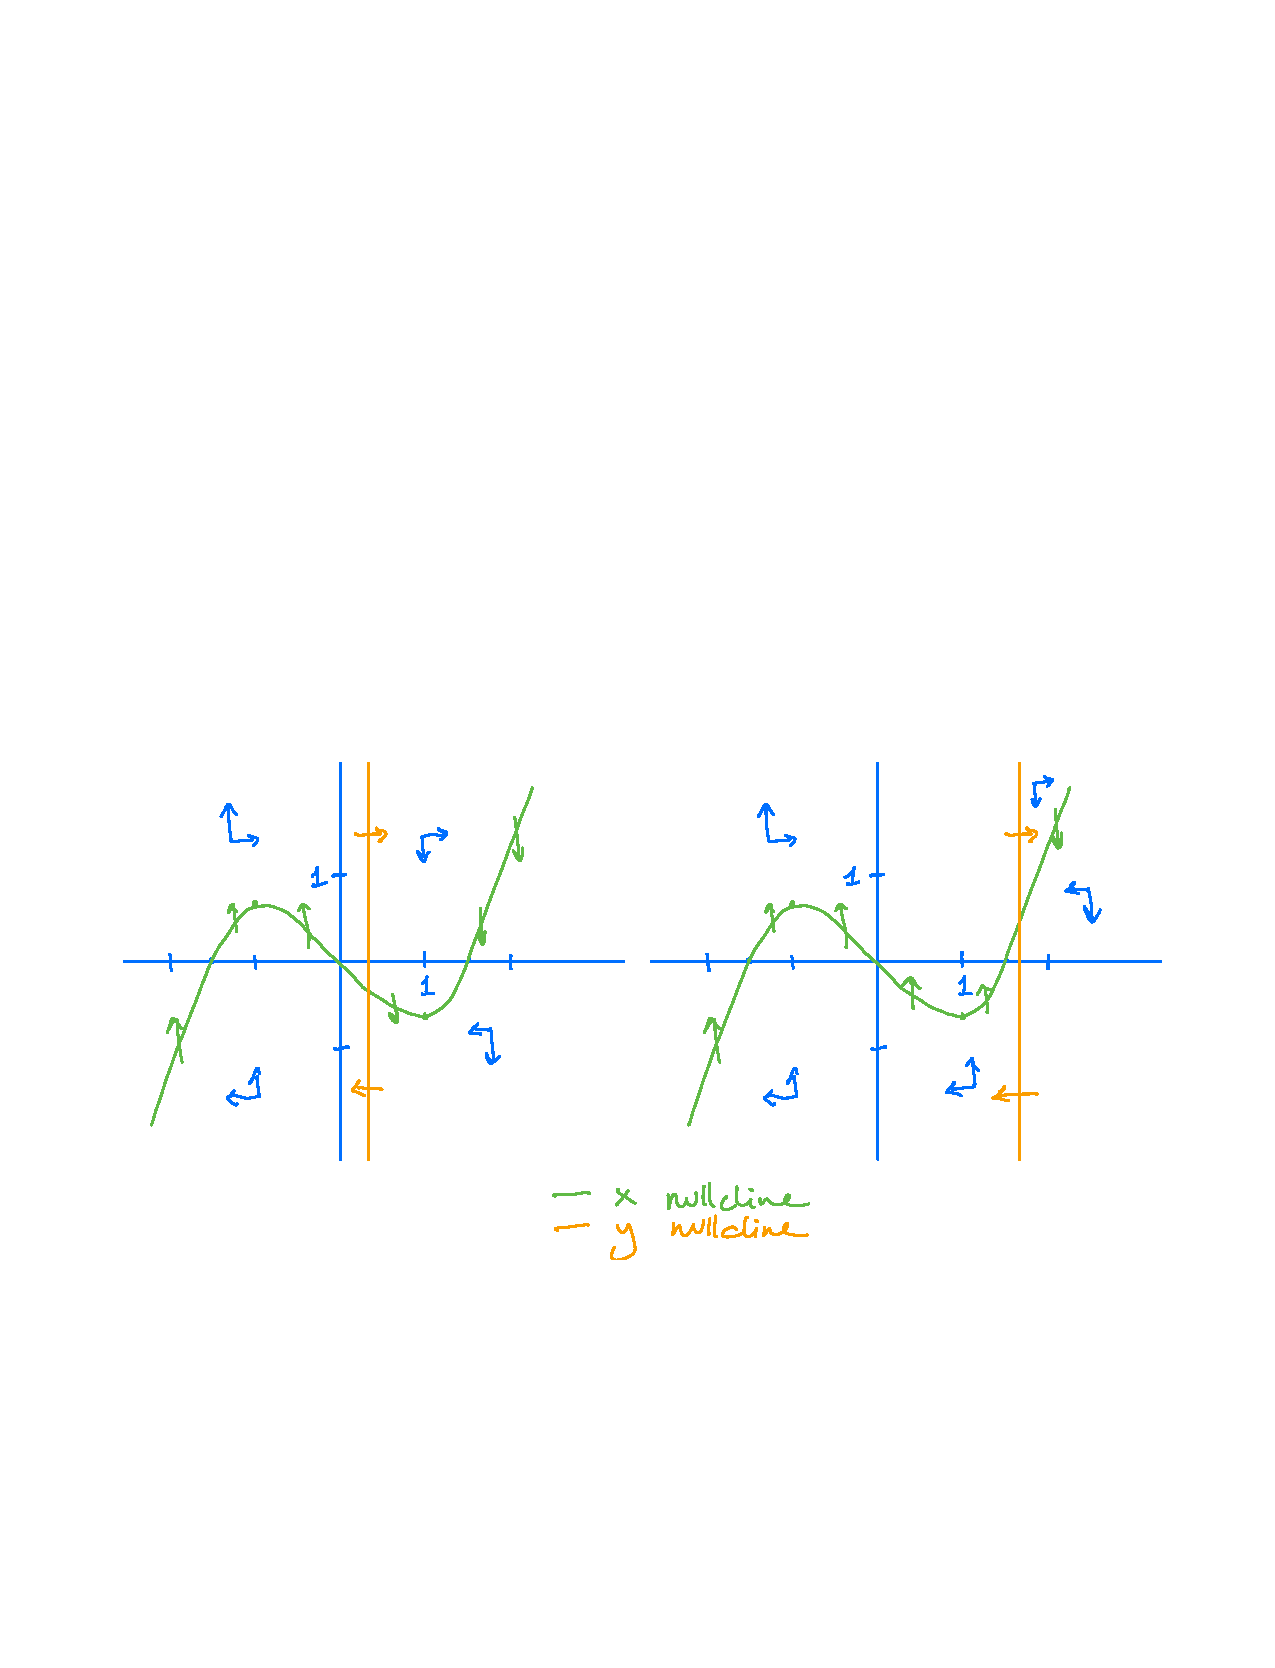
\includegraphics[width=6in]{img/H-07-3a}\\

The nullcines intersect exactly once.  The generic flow dictated by the nullclines seems to indicate clockwise rotation in the vector field.
\end{solution}

\item Find the fixed points and classify them as stable, unstable, or saddle points. Argue that if (and only if) the nullclines intersect on the middle branch of the cubic nullcline, the corresponding fixed point is unstable (reference your work in part a).


\begin{solution}
Fixed points when $a = x$ ($\dot y = 0$) and $y = a^3/3 - a$ ($\dot x = 0$) so there is a single fixed point at $(a,a^3/3 - a)$.

Classification: the Jacobian is
$\left(\begin{array}{c c}
\mu(1-x^2) & \mu \\
-1/\mu & 0
\end{array}\right)$.  At the fixed point, $\left(\begin{array}{c c}
\mu(1-a^2) & \mu \\
-1/\mu & 0
\end{array}\right)$.  Trace is $1-a^2$ and determinant is $1$ so the fixed point is never a saddle point.

Attractor / stable when $\vert a\vert > 1$ and repeller / unstable when $\vert a \vert < 1$.

The fixed point is unstable for $-1 < a < 1$, so when the $\dot y$ nullcline is a vertical line falling between $x= -1$ and $x = 1$.

The cubic nullcline is $y = x^3/3 - x$.  Its extrema occur when $x$ is given by $x^2 - 1 = 0$ so at $x = \pm 1$.  The middle branch of the cubic nullcline is the section where $-1 < x<1$.

If the nullclines intersect on the middle branch then $-1 < x < 1$ for the intersection with $x = a$ so $-1< a< 1$ and the fixed point is unstable.

If the fixed point is unstable then $-1<a<1$ and the vertical nullcline is given by $x=a$ so the vertical nullcline will intersect the cubic nullcline with $-1 < x<1$ (on the middle branch).
\end{solution}

\part Assume $\mu\gg 1$, show that the system has a stable limit cycle when $\vert a \vert < 1$.

\emph{Do this by constructing a trapping region that satisfies the Poincar\'e-Bendixson theorem.}

\emph{Remember that trapping regions for the Poincar\'e-Bendixson theorem need to be closed sets, so they need to include their boundary lines and points.}

\begin{solution}
\textbf{Constructing a trapping region is not a unique process.  It is likely that you created something far different to what I have here.  That is fine.}\\

Here we are really going to rely on the fact that $\mu\gg 1\gg1/\mu$.  Notice that this means that the vector field is \emph{much stronger} in the $x$ direction than in the $y$ direction, so away from nullclines, the vector field will be almost horizontal.\\

Frequently, it is advantageous to use translations of the nullclines to help you.  For example, notice that on the curve $y=-x+x^3/3+4/3$ the vector field always points to the right and the $x$ component of the vector field is $4\mu/3$.  Similarly on the curve $y=-x+x^3/3-4/3$ the vector field always points to the left and the $x$ component of the vector field is $-4\mu/3$.\\

Now we can't use these lines exactly for the outer boundary of our trapping region, but they are going to form part of the boundary.  Let's focus on the curve $y=-x+x^3/3+4/3$ to start. On the part of this curve from $x=-\infty$ to $x=1$, the vector field points to the right and up.  The slope of the curve is this region is always positive with magnitude $-1+x^2$.  The slope of the vector field is given by $\dot y/\dot x=\frac{(a-x)/\mu}{4\mu/3}=3(a-x)/4\mu^2$. Since $1\gg 1/\mu\gg1/\mu^2$ we have $3(a-x)/4\mu^2\ll a-x$ so that the slope of the curve is much more steep than the vector field and the vector field points in along the curve. \\

Notice that we have an issue on the region between $x=-1$ and $x=a$ where the vector field points to the right and up, i.e. out of the region.  To fix this, we are going to take a straight line with slope 1 from the point $(x,y)=(-1,2)$ on our curve (the local max) to the $y$ nullcline at $x=a$.  Because this line is above the curve $y=-x+x^3/3+4/3$, the $x$ component of the vector field is greater than $4\mu/3$.  Because $x$ is between $-1$ and $a$, the $y$ component of the vector field is between $(a+1)/\mu$ and $0$. Since $|a|<1$, we know that $(a+1)/\mu<2/\mu$.  Then the slope of the vector field is always between $0$ and $3/(2\mu^2)\ll 1$ and the vector field points in across this line.\\

As we cross the $y$ nullcline from left to right, the vector field points down, so we can take the straight line from $(a,3+a)$ all the way to the lower curve $y=-x+x^3/3-4/3$.\\

We would then repeat the argument on the lower parts of the curve.  See the sketch below.\\

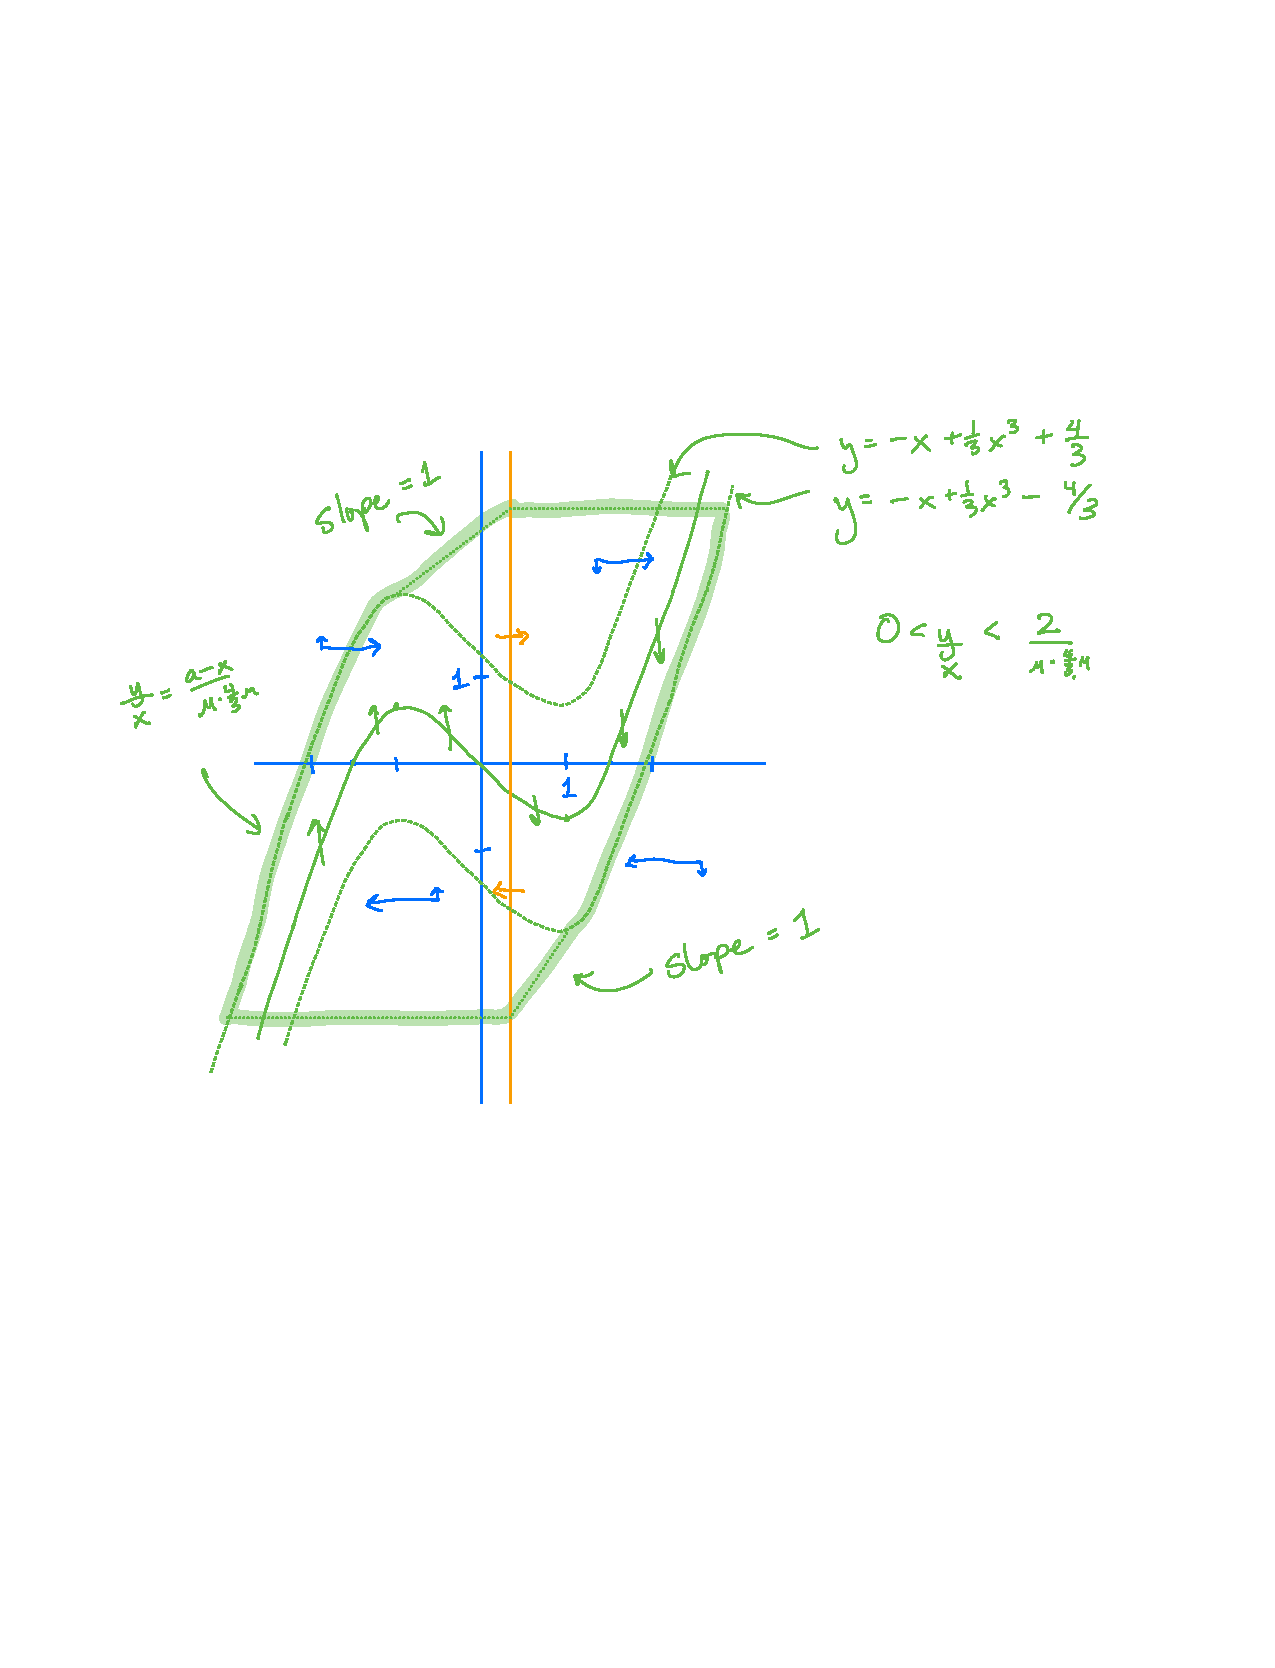
\includegraphics[width=4in]{img/H-07-3c}

For the inner boundary, we note that the equilibrium for $|a|<1$ is unstable, so we puncture the region at the equilibrium.
\end{solution}

\part Provide reasoning about flow in the system to argue that there cannot be a limit cycle when $a > 1$.

\begin{solution}
Consider an initial condition of the star in the figure (shown in blue).  The vector field dictates that the trajectory will move left and up until it intersects the $x$ nullcline at which point it will start moving up and to the right.  Because the $x$ direction dominates the flow, we move mostly horizontally except when we're close to the nullcline.  Close to the $x$ nullcline,  the $x$ component of the vector field is also small, and we move very close to (almost tangent to) the nullcline.  \\

We leave the nullcline near the maximum of $(-1,2/3)$ and again the horizontal component dominates and we move mostly horizontally, certainly with a slope less steep than 1 (see previous answer).  When we cross the $y$ nullcline we start moving down until we hit the $x$ nullcline.\\

When we hit the $x$ nullcline again, the same argument as before holds and we travel very close to the nullcline until we reach the $y$ nullcline again.  Crucially, this happens before we hit the local minimum, so we stay very close to all the nullclines and converge down to the equilibrium.  See sketch:

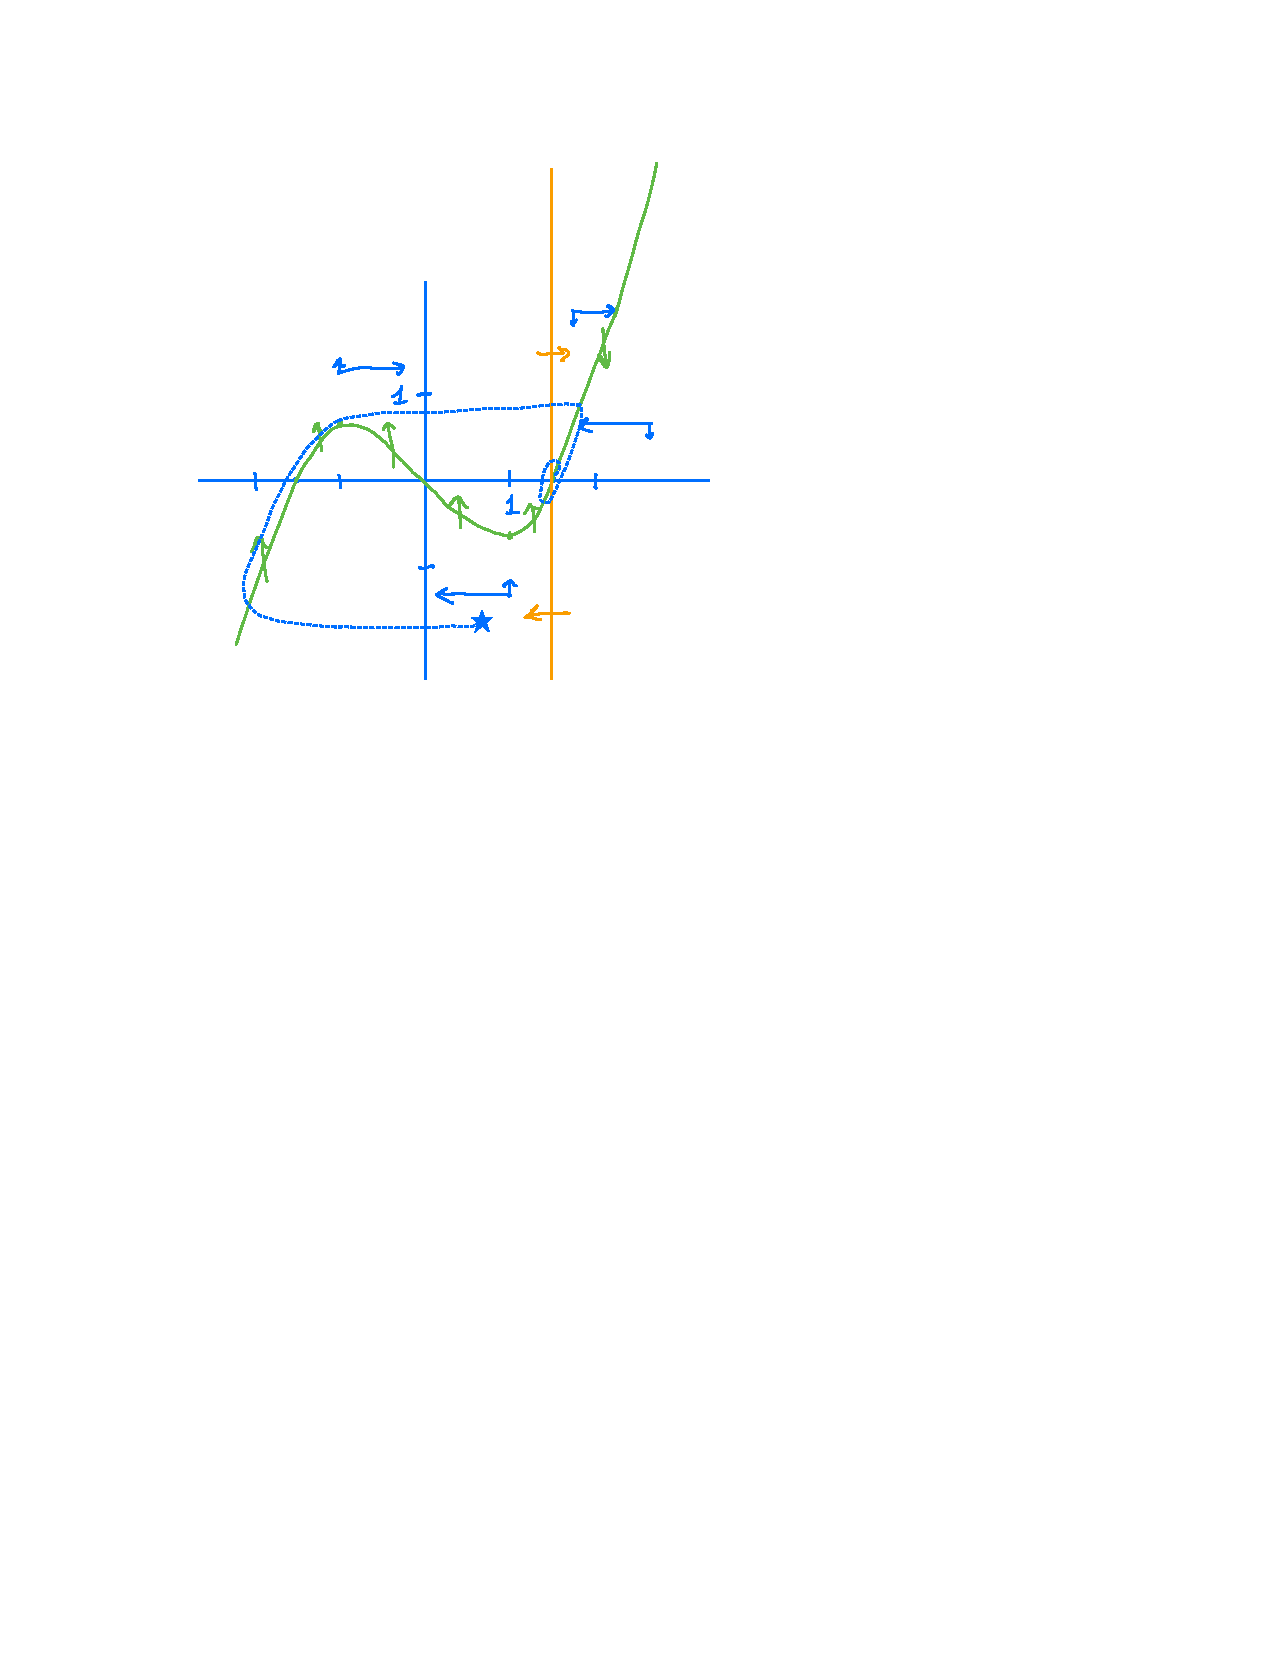
\includegraphics[width=3in]{img/H-07-3d}

\end{solution}


\part To model an excitable system in 4.5.3, we chose a parameter value where oscillation was turned off (we could not flow around the whole circle) and where we were close to the saddle node bifurcation.  We'll do a similar thing here.  Choose $a$ slightly greater than $1$.  

\begin{itemize}
    \item Describe how the system is \emph{excitable} (that it has a globally attracting fixed point, but certain disturbances can send the system past a ``threshold'' and on a long excursion through phase space before returning to the fixed point) and explain how excitability manifests in this system.
    \item Plot a phase portrait of the system with a trajectory showing the long excursion superimposed.  \emph{Remember to submit screenshots of your work on Gradescope}. 
    \item In addition, plot $x$ vs time for two cases, one where a disturbance leads to a long excursion and one where it does not.
\end{itemize} 

\begin{solution}
When $a>1$, the equilibrium is an attracting spiral and there are no limit cycles in the system (see above answer).  This is the rest state.\\

A small disturbance near the rest state can cause a large excursion.   Once near the fixed point, a small disturbance may lead to a trajectory that spirals in to the fixed point or that approaches the right branch of the nullcline and returns to the fixed point.  Specifically, if I perturb the initial conditions away from the fixed point a small amount or in a direction above the dx/dt = 0 nullcline, then the trajectory returns to the fixed point directly. \\

A disturbance that pushes that perturbs the initial condition so that it falls enough below the nullcline, leads to an excursion.  In this case, a particle  is pushed across to the left branch of the nullcline, climbs the left branch to the fold, is pushed across to the right branch, and then travels down the right branch to approach the fixed point.\\

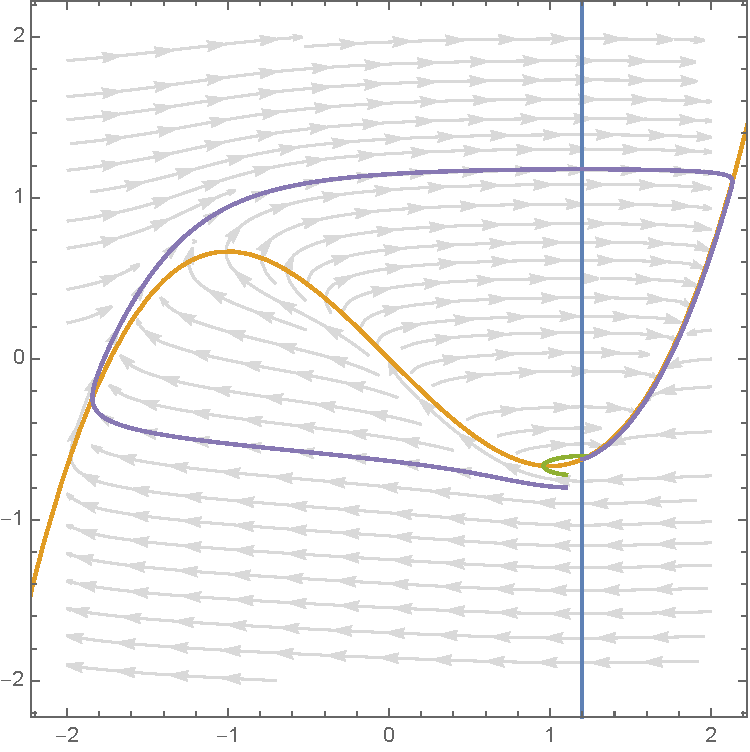
\includegraphics[width=2in]{img/H-07-3e-01}
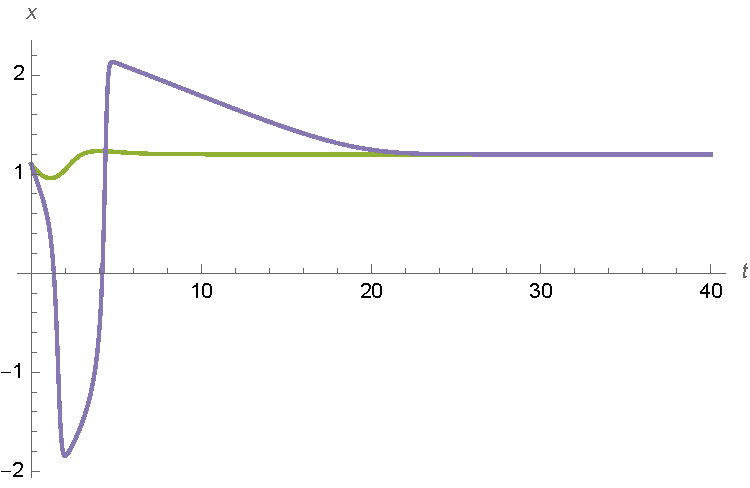
\includegraphics[width=3.5in]{img/H-07-3e-02}

The $x$-coordinates of the two trajectories are shown above right.  The green one returns to the fixed point in a straightforward way while the purple one goes on an excursion first.
\end{solution} 

Prof. Strogatz relates these models of excitability to neural systems.  Notice that the spike size (plot $x$ or $\theta$ with its excursion) doesn't depend on the size of the stimulus (so long as the stimulus exceeds some threshold).  The forced van der Pol model is related to the Fitzhugh-Nagumo model of neural activity. 
\end{parts}

% \question (7.2.18) Consider the predator-prey model 
% \begin{align*}
% \dot{x} = & r x (1-x/2) -\frac{2x}{1+x}y \\
% \dot{y} = & -y + \frac{2x}{1+x} y \\
% & r>0 \quad x,y\geq 0
% \end{align*}
% \begin{parts}
% \item What is the long term behavior of each population in the absence of the other?  Which species is the predator and which is the prey?  How do you know?
% \item Working analytically or in Mathematica, find the fixed points of the system. Use Mathematica to classify these fixed points as stable/unstable/saddle points based on their trace and determinant.  Include the trace / determinant info in your writeup.  In addition, plot the points on axes that have appropriate labels and unit markings.

% \emph{Some code to help with plotting, or you can work by hand:} 
% \begin{verbatim}
% f[x_,y_] = {r x (1-x/2) -(2x y)/(1+x), -y + (2x y)/(1+x)}
% soln = Solve[f[x, y] == 0, {x, y}]
% r0 = 5;
% ListPlot[{x, y} /. soln /. r -> r0, 
%  Ticks -> {Automatic, {{0, 0}, {r0/4, r/4}, {r0/2, r/2}, {3 r0/4, 
%      3 r/4}, {r0, r}}}, PlotStyle -> PointSize[Large]]
% \end{verbatim} 
% \item Explain the fixed points in the context of the problem.  What does each fixed point represent in the context of the problem and what seems to be the long term behavior of the system?
% \item According to index theory, what constraints are there on limit cycles in this system?
% \item Try to use the Bendixson criterion to show that there are not limit cycles in the system.  Find the curve(s) on which $\displaystyle\nabla\cdot \left(\begin{array}{c} \dot{x} \\ \dot{y}\end{array}\right) = 0$, write it/them in the form $y = h(x)$.  Explain why this criterion does not rule out limit cycles.
% \item Now try rescaling the vector field to see if we can use Dulac's criterion to rule out limit cycles.  Rescale the vectors in the vector field using a function of the form $\displaystyle g(x,y) = \frac{1+x}{x}y^{\alpha-1}$.  Make a suitable choice of $\alpha$ so that you can use Dulac's criterion to rule out limit cycles.

% \end{parts}

\question (inspired by 8.1.6) Consider the system
\begin{align*}
\dot{x} = &\ y - 2x \\
\dot{y} = &\ \mu+x^2-y.
\end{align*}
\begin{parts}
\item Sketch the nullclines.
\begin{solution}
The $\dot{x} = 0$ nullcline is a straight line (in black) and the $\dot{y} = 0$ nullcline are parabolas (in blue) drawn for three different values of $\mu$.  These $\mu$ values
are below, at, and above the bifurcation point.


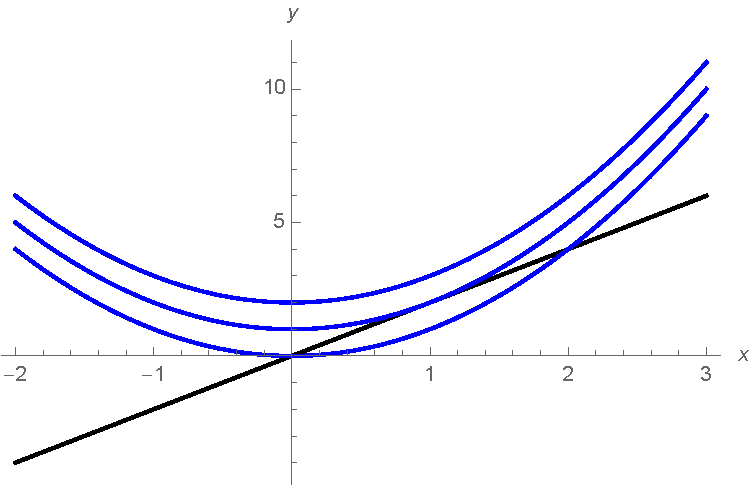
\includegraphics[width=2.5in]{img/C15nullclines.pdf}

\end{solution}
\item Find and classify the bifurcations that occur as $\mu$ varies.

\begin{solution}
To find and classify the bifurcations we need to identify the fixed points and find where the number of fixed points changes.
We can see from the nullclines that the black and blue lines intersect in two places for some values of $\mu$, and as $\mu$ increases
they intersect at a single point and then no points.  This means there's a saddle-node bifurcation.  So I've classified the bifurcation just
from looking at the nullcline picture.  To find the bifurcation, I suppose I need to find the point where there's just one fixed point, or, I can
find one of the fixed points and identify where it changes stability.  Either option would work.

At the fixed points $y = 2x$ and $y = \mu + x^2$ because $y-2x = 0$ and $\mu + x^2 - y = 0$.
This means $2x = \mu + x^2$ so $x^2 - 2x + \mu = 0$.  Using the quadratic formula,
\[x_\pm = 1 \pm \frac{1}{2} \sqrt{4 - 4\mu} = 1\pm \sqrt{1 - \mu}.\]
So there is just a single fixed point when $\mu = 1$ and for $\mu >1$ there are no fixed points.  Thus the bifurcation occurs
when $\mu = 1$ % at the point $(1, 2)$.
\end{solution}

\item Show that at the point of bifurcation the $\dot{x}=0$ and $\dot{y}=0$ nullclines are tangent.  

\begin{solution}
The slope of the $\dot{x} = 0$ nullcline of $y = 2x$ is $2$.  We want to show the other nullcline has the same slope at the point
of bifurcation.  The other nullcline is $y = x^2 + \mu$ so its slope is given by $2x$ and at the bifurcation point, $x = 1$, so its slope is also 2.
The two lines intersect at $(1,2)$ for $\mu = 1$ and they have the same slope, so they are tangent.
\end{solution}

\item Do you expect this to usually be true for a saddle-node bifurcation?  What about for a transcritical or pitchfork bifurcation?

\emph{When you think about this, assume the nullclines are smooth curves without sharp corners.}

\begin{solution}
Assume we have two nullclines that are continuous and differentiable.  At the bifurcation, they need to intersect in a single point, while just before (or just after) the bifurcation they need to intersect in multiple nearby points.  I'm assuming the nullclines are smooth curves (without sharp corners), so the nullclines will be tangent at the bifurcation.

We can also use the Jacobian to make an argument for tangency (the rows are linearly dependent at the bifurcation so the linear approximation to each nullcline is the same, i.e. they are tangent).
\end{solution}
\end{parts}

\question (ruling in or out limit cycles) For each of the following systems, 
\begin{itemize}
    \item Make a streamplot with two trajectories superimposed.
    \item Show there exists a closed trajectory, or show/argue that there cannot be a closed trajectory.
    
    \emph{You may need to reverse time, by studying the system $\dot x = -f(x,y), \dot y = -g(x,y)$ instead of the system $\dot x = f(x,y), \dot y = g(x,y)$.}
\end{itemize}  
\begin{parts}
    \item $\dot x = x - 2y - x^3, \dot y = 2x - y - y^3$
    \begin{solution}

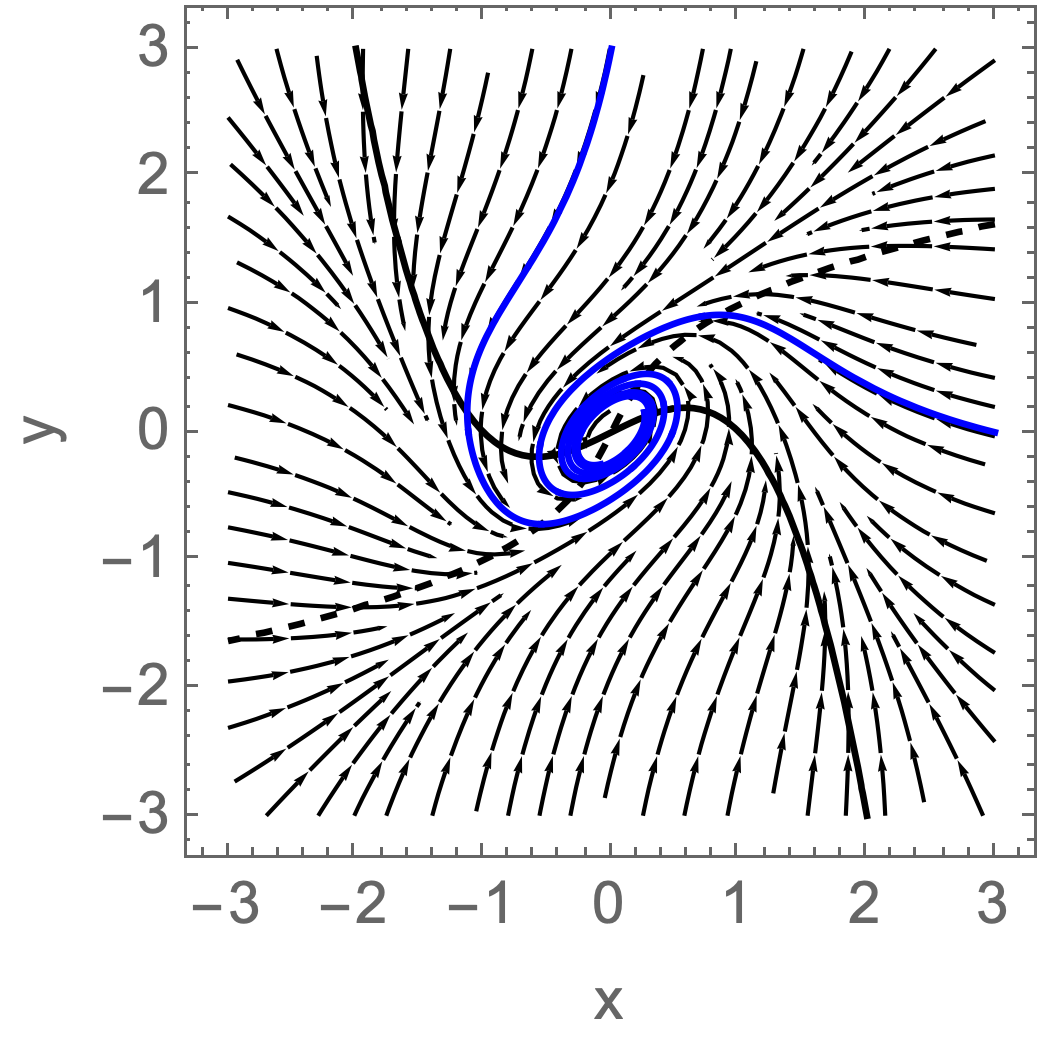
\includegraphics{img/PS07-S23-1.png}
    
It looks like there are no closed trajectories from the phase portrait, but it is a little hard to tell.  If you increase the integration time the trajectories spiral inward more, suggesting no closed trajectories.
    
Try Bendixson's: $f_x + g_y = 1 - 3x^2 -1-3y^2 = -3x^2 - 3y^2$.  This is negative everywhere but the origin, so an integral over a region of this quantity cannot be zero.  Closed trajectories are ruled out.


    
    \end{solution}
    \item $\dot x = -2x-y + x^3, \dot y = x - 2 y + y^3$
    \begin{solution}

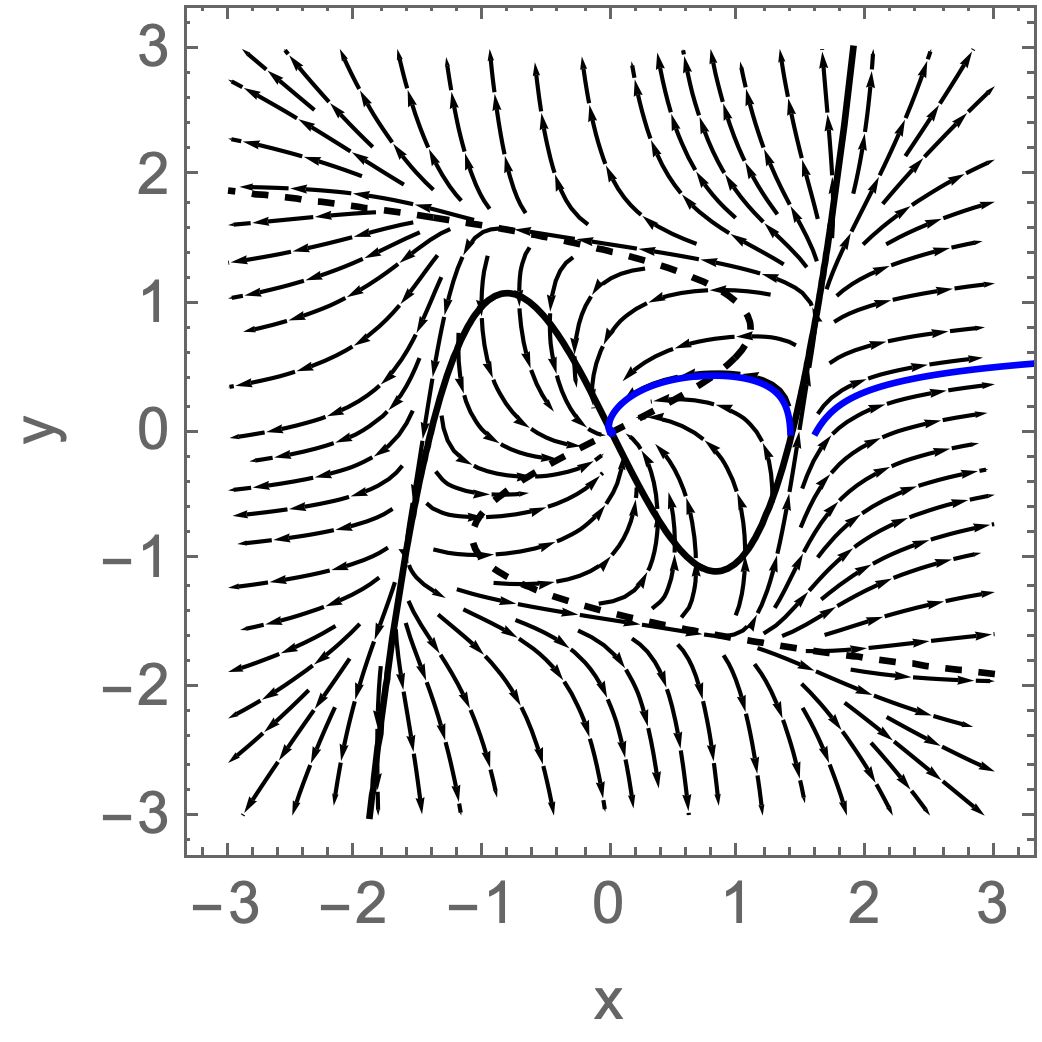
\includegraphics{img/PS07-S23-2.png}
    
It looks like there is an unstable limit cycle from the phase portrait.  Reverse time to make it stable: $\dot x = 2x+y - x^3, \dot y = -x + 2 y - y^3$.

From the plot there is one fixed point and it is at the origin.  Working in reversed time: Jacobian: $\left(\begin{array}{c c} 2 - 3x^2 & 1 \\ -1 & 2- 3y^2 \end{array}\right)$.  At the origin this is $\left(\begin{array}{c c} 2 & 1 \\ -1 & 2 \end{array}\right)$.  Trace is $4$, determinant is $5$ so repeller.

To create an outer trapping region (that we can then puncture), $-x^3$ and $-y^3$ should dominate the linear terms for large enough $x$ and $y$, so try a box with $x = \pm 10$, $y=\pm 10$.  The max/min value of $2x+y = \pm 30$ and the max/min value of $-x+2y = \pm 30$ while $-x^3 = \mp 1000$ and $-y^3 = \mp 1000$.  So $\dot y < -900$ when $y = 10$ and $\dot y > 900$ when $y = -10$.  That guarantees flow is inward on the horizontal boundaries.  Similar limits for the vertical boundaries.

We have a trapping region.  We puncture it by excluding a small open circle about the repelling fixed point, and we have a closed region that traps all trajectories that start within it, so we have a closed trajectory by the Poincare-Bendixson theorem.


    
    \end{solution}
    \item $\dot x = 2x-y-4x^3, \dot y = -x + 2y + 4y^3 $ 
    \begin{solution}

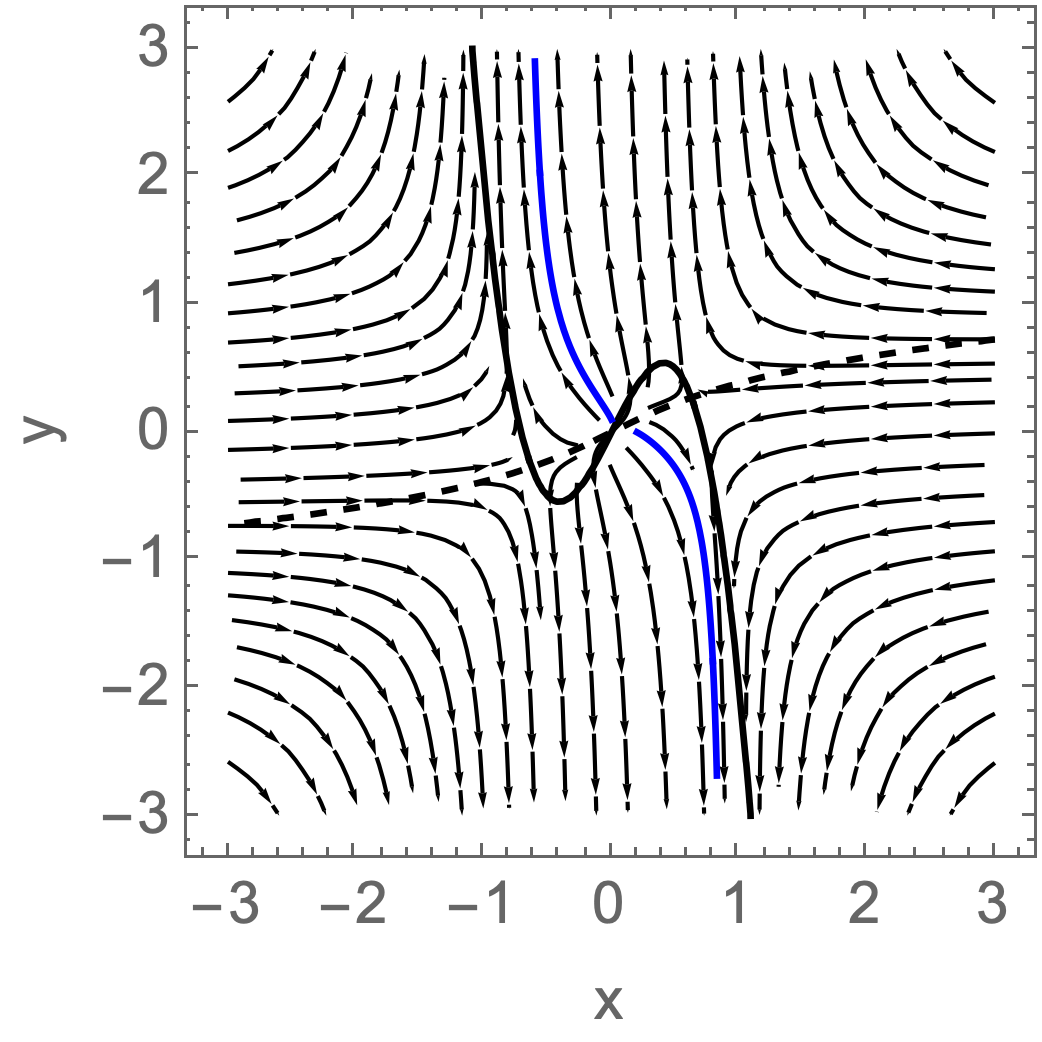
\includegraphics{img/PS07-S23-3.png}
    
It looks like there are no closed trajectories from the phase portrait.
    
Try Bendixson's: $f_x + g_y = 2 - 12x^2 +2 +12y^2 = 4 - 12x^2+12y^2$.  This takes on multiple signs.  Can't rule out closed trajectories.

Check if it is a gradient system: If $\dot x = -V_x$ and $\dot y = -V_y$ then $\partial_y \dot x = -V_{xy}$ and $\partial_x \dot y = -V_{yx}$.

$\partial_y \dot x = -1$.  $\partial_x \dot y = -1$.  These are equal.  This is a gradient system.  The gradient is
$V(x,y) = -\int (2x-4x^3-y)dx + c_1(y) = x^2 - x^4 -xy + c_1(y)$.

$V(x,y) = -\int (-x + 2y + 4y^3)dy + c_2(x) = -xy + y^2 + y^4 + c_2(x)$.

Reconciling these, $V(x,y) = -x^2 + x^4 + xy - y^2 - y^4$ is a potential function so there are no closed trajectories.
    
    \end{solution}
\end{parts}



\question (optional: Weakly nonlinear systems)

Consider a system of the form $\ddot x + x + \epsilon h(x,\dot x) = 0$ with $\epsilon$ small.

\begin{parts}
\item For the 2nd order linear system $\ddot x + x = 0$, create a first order system of equations, $\dot x = y, \dot y = ?$.  This is a linear system.  Classify the fixed point.
\item This system is conservative (it is of the form $\ddot x = F(x)$).  Find the conserved quantity and sketch a phase portrait of the system.
\item Show that $x(t) = A\cos t$, $y(t) = \dot x = ?$ is a trajectory of the system.  \emph{Show that it satisfies the differential equations.}
\item Let $E(x,y) = \dfrac{1}{2}x^2 + \frac{1}{2}y^2$.  Find $\dfrac{dE}{dt}$ for the system $\ddot x + x + \epsilon h(x,\dot x) = 0$ (where $\dot x = y$) with the following $h$ functions:
\begin{itemize}
    \item $h(x,y) = xy^2$
    \item $h(x,y) = (x^2-1)y^3$
\end{itemize}
\item In the $\ddot x + x = 0$ system, the period of cycles is $T = 2\pi$, and $x(t) = A\cos t, y(t) = -A\sin t$ is a solution for any $A$.  

In the weakly nonlinear system, assume there exists a limit cycle that is preserved from the linear system.  It would be of the form $x(t) = A\cos t$ with period $T\approx 2\pi$.  We want to find the value of $A$ associated with the limit cycle.  

$\Delta E = \int_0^T \frac{dE}{dt}dt \approx -\epsilon \int_0^{2\pi} h(x(t),y(t))y(t)dt$

Substitute $x(t) = A\cos t$ and $y(t) = -A\sin t$.  On a closed trajectory, $\Delta E = 0$. 


\item Find the radii associated with closed trajectories (the values of $A$ where $\Delta E = 0$).
\item Use Mathematica/Python to create a phase portrait with three trajectories superimposed.  If relevant, one trajectory should spiral inwards towards a stable limit cycle and another should spiral outwards.  The third trajectory should be chosen to match the radius of the closed trajectory you found in your calculation.  \emph{If not relevant, plot three trajectories of your choice.}
\end{parts}
% Remember to submit screenshots of your work.% as well as the source code.
% \item By modifying the Mathematica code provided, use an approximate Poincar\'e map to attempt to confirm (or amend) your work in (a).

% \emph{Using Mathematica, we approximate the Poincar\'e map (at a few values of the domain) numerically, rather than exactly finding the map analytically.}
% \end{parts}

% \item Let $h(x,\dot x) = (1-x^2)\dot x$ for the system $\ddot x + x + \epsilon h(x,\dot x) = 0$.  This is very similar to the system we analyzed in class.
% \begin{parts}
% \item Derive the 2d first-order system associated with this problem.  In addition, create the backwards time version of this system.

% \emph{To create a backwards time version, reverse time in the system by doing a change of variables where $t\rightarrow -t$.  Perhaps let $\tau = -t$, so that the backwards time system is $\dfrac{dx}{d\tau}, \dfrac{dy}{d\tau}$.}
% % \item Create plots of the approximate Poincar\'e maps for the forwards time and backwards time systems. 
% % \item Describe how you can identify the stability of the limit cycle using information in the approximate Poincar\'e map, and identify the stability of the limit cycle in the forwards time and backwards time systems.
% \item Create streamplots of the two systems, each with a trajectory superimposed.  To select the trajectories, start in the backwards time system and generate a trajectory with initial conditions that start outside of the limit cycle.  Read off the final state value for that trajectory, and use that final value as the initial condition for generating a trajectory in the forward system.


% Accessing the final state value: \begin{verbatim}
% finalpt = {x[t],y[t]}/.soln2b/.t->tMax
% x00 = finalpt[[1,1]]
% y00 = finalpt[[1,2]]
% \end{verbatim}


% \begin{itemize}
% \item What is the relationship between the two trajectories that you have generated?
% \item For the forward time system, what makes it necessary to choose the initial conditions carefully?  \emph{What happens if you start outside of the limit cycle and don't choose initial conditions in this way?}
% \end{itemize}


% \end{parts}




\end{questions}

\vfill

\noindent\textbf{March 22} (Wednesday) project topic + team preferences submitted during class

\noindent\textbf{March 24} (Friday) teams assigned (usually teams of 3)

\noindent\textbf{March 31} (Friday) project proposal

\noindent\textbf{Weekly on Fridays in April} Individual project work log due: this is the core individual deliverable of the project work.

\noindent\textbf{April 19} (Wednesday) team progress report slides due

\noindent\textbf{April 21/24/26} (Friday/Monday/Wednesday) team progress report presentations

\noindent\textbf{May 10, 9am} (Wednesday) team final presentation slides due

\noindent\textbf{May 10, 2pm-5pm} (Wednesday) team final presentations; final individual log due



\end{document}
